\noindent \textbf{\LARGE 从理论到实现}\vspace{8pt}\\
\noindent \textbf{\Huge 基于物理的渲染}\qquad\textbf{\large 第三版}\vspace{8pt}\\
\noindent \textbf{\large 原著 \quad Matt Pharr, Wenzel Jakob \& Greg Humphreys}\vspace{5pt}\\
\noindent \textbf{\large 翻译 \quad Kanition}\vspace{12pt}\\

\noindent {\bfseries 英文原版}

\noindent Copyright \copyright\ 2004-2024 Matt Pharr, Wenzel Jakob, and Greg Humphreys

\noindent 官方网址:\url{https://www.pbr-book.org}\\

\noindent {\bfseries 本中译版}

\noindent Copyright \copyright\ 2021-2024 Kanition

\noindent 更新网址:\url{https://github.com/kanition/pbrtbook}

\noindent {\ttfamily\small\input{ver_info.txt}}\\

\noindent {\bfseries 许可协议}\raisebox{-0.1\height}{
    $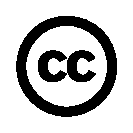
\includegraphics[height=10pt]{Pictures/preface/cc.eps}$
    $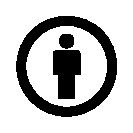
\includegraphics[height=10pt]{Pictures/preface/by.eps}$
    $
\includegraphics[height=10pt]{Pictures/preface/nc.eps}$
    $
\includegraphics[height=10pt]{Pictures/preface/sa.eps}$}

\noindent \href{https://creativecommons.org/licenses/by-nc-sa/4.0/}
{Creative Commons Attribution-NonCommercial-ShareAlike 4.0 International}

\noindent \href{https://creativecommons.org/licenses/by-nc-sa/4.0/deed.zh-hans}
{知识共享署名—非商业性使用—相同方式共享4.0国际公共许可协议}

\noindent {\small{详见:\url{https://creativecommons.org/licenses/by-nc-sa/4.0/legalcode.zh-hans}}}\\


{\itshape
本中译版(以下简称“本书”)系译者(笔名 Kanition)自学英文经典书籍
《Physically Based Rendering: From Theory To Implementation》第三版时自行翻译而成。
使用本书及其源码须遵循相关许可证协议。

本书在翻译时遵照原书编排,译文尽力保留了原文词句,但因笔者水平有限,
而原文长句极多,故可能会存在病句甚至误翻,请读者见谅并指正。

此外,笔者根据自己的学习情况对内容作了补充,
例如自行编写补充章节、在边栏进行注释解说、修正一些笔误等。
除补充章节外,行文中凡是笔者自行变动或增添过的地方都有“译者注”的标记。

原书在线版本以网页形式呈现,可以方便地展开、折叠示例代码。
本书虽受到PDF格式限制,但依旧精心保留了代码链接跳转功能,方便读者查阅。
若读者在实践中还有更多需求,建议参考原书所附代码库。

本书由{\scshape \LaTeX} 编写而成,源码已经发布在上述网址,欢迎访问获取最新版。

{\color{red}\sffamily{欢迎提出宝贵意见和建议。如果你发现本书存在错误,请一定要告诉我们!
讨论区:{\normalfont\url{https://github.com/kanition/pbrtbook/discussions}}}}
}